\definecolor{pyplotC0}{RGB}{31,119,180}
\begin{figure}[t!]
\centering
%
\begin{subfigure}{0.45\textwidth}
\centering
\documentclass{standalone}
\usepackage{tikz}

\begin{document}
\definecolor{pyplotC0}{RGB}{31,119,180}
\newcommand{\biquad}[1]{\protect\tikz[baseline=0ex]
  \protect\draw [draw=gray, very thick, scale=0.60, rounded corners=0.5mm]
  (0, 0) -- (#1, 0) -- (#1+0.25, 0.3) -- (1.25, 0.3) {};}
\newcommand{\shelf}{\protect\tikz[baseline=0ex]
  \protect\draw [ultra thick, scale=1, rounded corners=0.5mm, color=pyplotC0]
  (0, 0) -- (0.15, 0) -- (0.85, 0.6) -- (1, 0.6) {};}

\begin{plottikz}
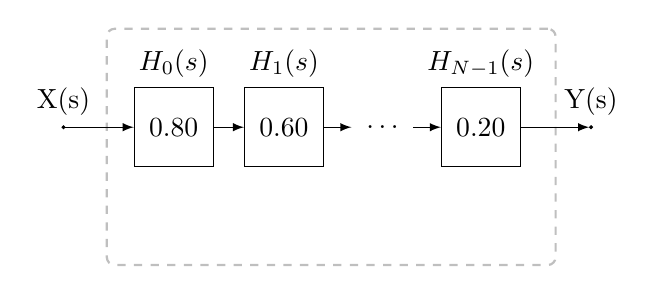
\begin{tikzpicture}
[scale=1, node distance=1.4cm, >=latex,
block/.style={
	rectangle, minimum size=10mm, minimum width=10mm, inner sep=2pt,
	draw=black},
largeblock/.style={
	rectangle, minimum size=8mm, minimum width=8mm, inner sep=3pt, thick,
	draw=gray!50, dashed, rounded corners=1mm},
dot/.style={
	circle, minimum size=1pt, inner sep=0pt,
	fill=black, draw=black}]

% coordinates
\coordinate (input) at (0, 0);
\coordinate [right of=input] (h0);
\coordinate [right of=h0] (h1);
\coordinate [right of=h1, node distance=2.5cm] (hN);
\coordinate [right of=h1, node distance=1.25cm] (dots);
\coordinate [right of=hN] (output);
\coordinate [right of=h0, node distance=2cm, yshift=-0.25cm] (cascade);

% input and output nodes
\node [dot, label={X(s)}] (In) at (input) {};
\node [dot, label={Y(s)}] (Out) at (output) {};

% cascade
\node [largeblock, minimum size=3cm, minimum width=5.7cm,
       label={[yshift=-2.85cm] \shelf}]
       (Cascade) at (cascade) {};

% biquads
\node [block, label={[yshift=0] $H_{0}(s)$}] (H0) at (h0) {\biquad{0.80}};
\node [block, label={[yshift=0] $H_{1}(s)$}] (H1) at (h1) {\biquad{0.60}};
\node [block, label={[yshift=0] $H_{N-1}(s)$}] (HN) at (hN) {\biquad{0.20}};


% signal flow
\draw [->] (In) -- (H0);
\draw [->] (H0) -- (H1) node [above, pos=0.5] {};
\draw [->] (H1.east) -- ++(0.35, 0) {};
\draw [<-] (HN.west) -- ++(-0.35, 0) {};
\draw [->] (HN) -- (Out) node [above, pos=0.5] {};
\node at (dots) {$\ldots$};

\end{tikzpicture}
\end{plottikz}

\end{document}

\caption{Signal flow for shelving filter cascade with input $X(s)$, output $Y(s)$ and
biquads $H_\mu(s)$ in series in the Laplace domain.}
\label{fig:tikz-cascade-biquads}
\end{subfigure}
%
\\\vspace{0.3cm}
%
\begin{subfigure}{0.45\textwidth}
\centering
\begin{plottikz}
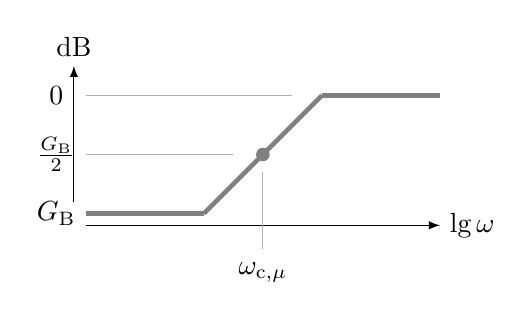
\begin{tikzpicture}[scale=1.5]
\draw [-latex] (0,-0.1) -- (3,-0.1) node [right]  {$\lg \omega$};
\draw [-latex] (-0.1,0.1) -- (-0.1,1.25) node [above]  {dB};
\draw [gray, ultra thick] (0,0) -- (1,0);
\draw [gray, ultra thick] (1,0) -- (2,1);
\draw [gray, ultra thick] (2,1) -- (3,1);
\draw[gray, fill=gray] (1.5,0.5) circle (1.5pt);
\node at (-0.25,1) {$0$};
\node at (-0.25,0.5) {$\frac{G_\mathrm{B}}{2}$};
\node at (-0.25,0) {$G_\mathrm{B}$};
\node at (1.5,-0.5) {$\omega_{\mathrm{c},\mu}$};
\node at (1,-0.25) {};
\node at (2,-0.25) {};
%
\draw [thin, black!30] (0,1) -- (1.75,1);
\draw [thin, black!30] (0,0.5) -- (1.25,0.5);
\draw [thin, black!30] (1.5,-0.3) -- (1.5,0.35);
%
\end{tikzpicture}
\end{plottikz}
\caption{Level response $20\lg |H_\mu(\omega)|$ of low-shelving
biquad for $G_\mathrm{B}<0$ and mid-level cutoff frequency $\omega_{\mathrm{c},\mu}$.
%The transition between the pass band and the shelving band can be somewhat controlled
%by $Q$, which then yields under-/overdamped responses.
}
\label{fig:schematic_magres_2nd_ls}
\end{subfigure}
%
\\\vspace{0.3cm}
%
\begin{subfigure}{0.45\textwidth}
\centering
\begin{plottikz}
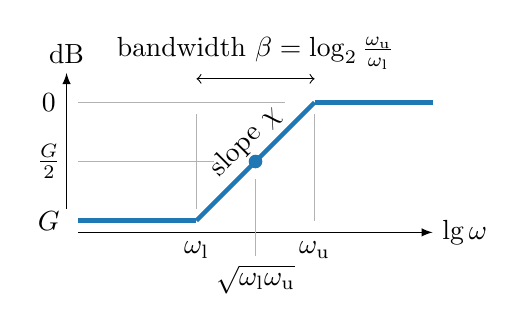
\begin{tikzpicture}[scale=1.5]
\draw [<->] (1,1.2) -- node [above] {bandwidth $\beta=\log_2{\frac{\omega_\mathrm{u}}{\omega_\mathrm{l}}}$}  (2,1.2) ;
\node [opacity=0] (first) {};
\node [draw=white, right of=first,rotate=45,anchor=north,xshift=1.5cm, yshift=0.2cm] {slope $\chi$};
%
\draw [-latex] (0,-0.1) -- (3,-0.1) node [right]  {$\lg \omega$};
\draw [-latex] (-0.1,0.1) -- (-0.1,1.25) node [above]  {dB};
\draw [color=pyplotC0, ultra thick] (0,0) -- (1,0);
\draw [color=pyplotC0, ultra thick] (1,0) -- (2,1);
\draw [color=pyplotC0, ultra thick] (2,1) -- (3,1);
\draw[color=pyplotC0, fill=pyplotC0] (1.5,0.5) circle (1.5pt);
\node at (-0.25,1) {$0$};
\node at (-0.25,0.5) {$\frac{G}{2}$};
\node at (-0.25,0) {$G$};
\node at (1.5,-0.5) {$\sqrt{\omega_\mathrm{l} \omega_\mathrm{u}}$};
\node at (1,-0.25) {$\omega_\mathrm{l}$};
\node at (2,-0.25) {$\omega_\mathrm{u}$};
%
\draw [thin, black!30] (0,1) -- (1.75,1);
\draw [thin, black!30] (0,0.5) -- (1.15,0.5);
\draw [thin, black!30] (1.5,-0.3) -- (1.5,0.35);
\draw [thin, black!30] (2,0) -- (2,0.9);
\draw [thin, black!30] (1,0.1) -- (1,0.9);
%
\end{tikzpicture}
\end{plottikz}
\caption{Level response $20\lg |H(\omega)|$ of shelving filter cascade
for $G<0$ and lower/upper cutoff frequency $\omega_\mathrm{l/u}$. For a dedicated
$\omega_\mathrm{u}$,
additionally two of the three parameters $\chi$, $\beta$ and $G$ can be freely
adjusted.}
\label{fig:schematic_magres_2nd_arb}
\end{subfigure}
%
\caption{Signal-flow graph (a) and schematic level responses of a single 2nd
order shelving filter (b) and the proposed shelving filter cascade (c).}
\label{fig:schematic_magres}
\end{figure}
